\section{Results}\label{sec:results}

\subsection{Primary specification (H1)}

Before enactment, a USD~10\,bn five-day inflow is associated with a 3-month yield \bPre{}\,bp lower after ten business days (s.e.~\bPreSE{}; 90\% CI \bPreLo{} to \bPreHi{}). After enactment the estimate is \bPost{}\,bp (s.e.~\bPostSE{}; 90\% CI \bPostLo{} to \bPostHi{}; \bPostP{}). The difference is $\delta_{10}=\bDiff{}$\,bp (s.e.~\bDiffSE{}, \bDiffP{}). It is not statistically distinguishable from zero, and its sign is opposite to H1, which predicts $\delta_{10}<0$ (Table~\ref{tab:primary}). At the scale of~\cite{ahmed2025} the estimates are \bAnchorPre{}\,bp before and \bAnchorPost{}\,bp after enactment per USD~3.5\,bn; per standard deviation of~$F_t$ they are \bSDPre{} and \bSDPost{}\,bp. Dropping the same-day controls changes nothing material ($\delta_{10}=\bLagsDiff{}$\,bp, \bLagsDiffP{}). \textbf{H1 is not supported.}

Fig.~\ref{fig:irf} shows the full responses. Before enactment the response builds steadily, reaching \bTwPre{}\,bp at $h=20$. After enactment it bottoms out at \postTrough{}\,bp at $h=\postTroughH{}$ and then fades towards zero. The gap widens with the horizon ($\delta_{20}=\bTwDiff{}$\,bp, \bTwDiffP{}). No single horizon is significant at the 5\% level, and adjacent horizons are highly correlated by construction.

\begin{figure}[!t]
\centering
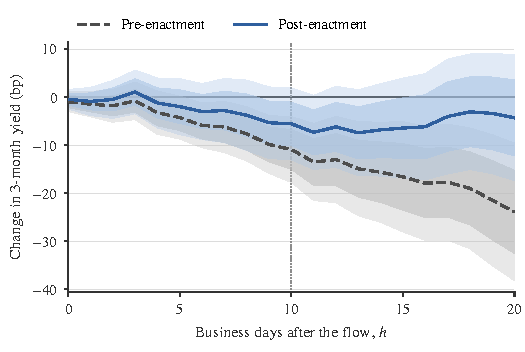
\includegraphics[width=\columnwidth]{figures/fig_irf.pdf}
\caption{Response of the 3-month bill yield to a USD~10\,bn five-day stablecoin inflow, before and after the GENIUS Act (Eq.~\ref{eq:lp}). Lines: point estimates; shaded: 68\% and 90\% Newey--West bands. Dotted line: the pre-registered horizon $h=10$.}
\label{fig:irf}
\end{figure}

\begin{table*}[!t]
\centering
\caption{Primary local projection: 3-month Treasury bill (pre-registered)}
\label{tab:primary}
\footnotesize
\begin{adjustbox}{max width=\textwidth}
% generated by src/viz/paper_tex.py
\begin{tabular}{lrrrrrrrr}
\toprule
 & \multicolumn{2}{c}{Pre-enactment $\beta_h$} & \multicolumn{2}{c}{Post-enactment $\beta_h+\delta_h$} & \multicolumn{2}{c}{Difference $\delta_h$} & & \\
\cmidrule(lr){2-3}\cmidrule(lr){4-5}\cmidrule(lr){6-7}
Horizon, scaling & est. (s.e.) & $p$ & est. (s.e.) & $p$ & est. (s.e.) & $p$ & $N_{pre}$ & $N_{post}$ \\
\midrule
$h=0$, per USD 10\,bn & \ensuremath{-}0.95 (1.25) & 0.45 & \ensuremath{-}0.45 (1.24) & 0.71 & +0.50 (0.80) & 0.53 & 1135 & 322 \\
$h=5$, per USD 10\,bn & \ensuremath{-}4.28 (2.70) & 0.11 & \ensuremath{-}1.98 (3.53) & 0.57 & +2.29 (3.00) & 0.45 & 1135 & 317 \\
$h=10$, per USD 10\,bn & \ensuremath{-}10.90 (4.16) & 0.01 & \ensuremath{-}5.56 (4.54) & 0.22 & +5.35 (5.21) & 0.30 & 1135 & 312 \\
$h=20$, per USD 10\,bn & \ensuremath{-}23.88 (8.69) & 0.01 & \ensuremath{-}4.31 (7.95) & 0.59 & +19.57 (11.02) & 0.08 & 1135 & 302 \\
$h=10$, per 1 s.d. (USD 1.81\,bn) & \ensuremath{-}1.97 (0.75) & 0.01 & \ensuremath{-}1.01 (0.82) & 0.22 & +0.97 (0.94) & 0.30 & 1135 & 312 \\
$h=10$, per USD 3.5\,bn & \ensuremath{-}3.82 (1.45) & 0.01 & \ensuremath{-}1.94 (1.59) & 0.22 & +1.87 (1.82) & 0.30 & 1135 & 312 \\
\bottomrule
\end{tabular}

\end{adjustbox}

\vspace{2pt}
\parbox{\textwidth}{\footnotesize Dependent variable: $y_{t+h}-y_{t-1}$ in bp. Coefficients scaled to the stated flow size; Newey--West standard errors ($h+1$ lags) in parentheses; two-sided $p$-values. $N_{post}$ falls with $h$ because leads run to the end of the sample.}
\end{table*}

\subsection{Term structure (H2)}

Before enactment the ten-day response shrinks with maturity: \tFourWPre{}\,bp at 4~weeks, \tThreeMPre{} at 3~months, \tSixMPre{} at 6~months, \tOneYPre{} at 1~year and \tTwoYPre{} at 2~years (Fig.~\ref{fig:term}, Table~\ref{tab:term}). Only the 3-month estimate is significant at 5\% (\tThreeMPreP{}; 4-week \tFourWPreP{}). The gradient is consistent with preferred-habitat demand~\cite{vayanos2021}, but it was already present before the Act. After enactment every tenor is smaller in absolute value and imprecise, and no tenor's $\delta_{10}$ is significant (all $p\geq\termDiffMinP{}$). \textbf{H2 is not supported.}

\begin{figure}[!t]
\centering
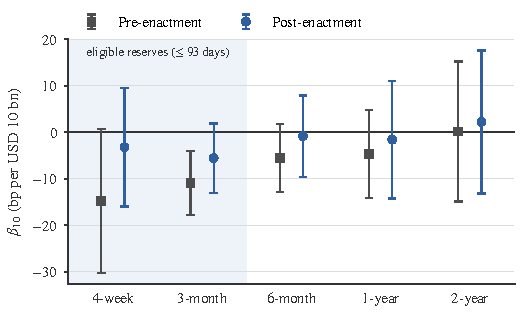
\includegraphics[width=\columnwidth]{figures/fig_term.pdf}
\caption{Ten-day response $\beta_{10}$ by tenor, per USD~10\,bn five-day inflow, with 90\% Newey--West intervals. Shaded: maturities eligible as reserves under \S4(a)(1)(A)(iii). Bills are secondary-market yields; 1- and 2-year yields are constant-maturity.}
\label{fig:term}
\end{figure}

\begin{table}[!t]
\centering
\caption{Term structure of $\beta_{10}$ (bp per USD 10\,bn, s.e.)}
\label{tab:term}
\footnotesize
\begin{adjustbox}{max width=\columnwidth}
% generated by src/viz/paper_tex.py
\begin{tabular}{lrrrr}
\toprule
Tenor & Pre $\beta_{10}$ & Post & $\delta_{10}$ & $p$ \\
\midrule
4-week bill & \ensuremath{-}14.78 (9.44) & \ensuremath{-}3.22 (7.75) & +11.55 (10.18) & 0.26 \\
3-month bill & \ensuremath{-}10.90 (4.16) & \ensuremath{-}5.56 (4.54) & +5.35 (5.21) & 0.30 \\
6-month bill & \ensuremath{-}5.56 (4.43) & \ensuremath{-}0.84 (5.33) & +4.73 (5.87) & 0.42 \\
1-year CMT & \ensuremath{-}4.65 (5.74) & \ensuremath{-}1.60 (7.71) & +3.05 (8.62) & 0.72 \\
2-year CMT & 0.14 (9.14) & 2.22 (9.35) & +2.08 (10.72) & 0.85 \\
\bottomrule
\end{tabular}

\end{adjustbox}
\end{table}

\subsection{Asymmetry (H3)}

Before enactment, outflows are associated with much larger yield moves than inflows (Fig.~\ref{fig:asym}, Table~\ref{tab:asym}). Per USD~3.5\,bn at $h=10$, an inflow is associated with \aInPre{}\,bp (\aInPreP{}) and an outflow with \aOutPre{}\,bp (\aOutPreP{}); equal slopes are rejected at \aEqPreP{}. This matches the direction of the first version of~\cite{ahmed2025}. The magnitude, however, is implausible: \aOutPreTw{}\,bp at $h=20$. Of the \outPre{} pre-enactment outflow days, \outPreHike{} fall in 2022--23, when the Federal Reserve was raising rates. Stablecoins pay no interest, so rising rates plausibly caused both the redemptions and the rise in yields. We read this asymmetry as rate-driven redemption, not fire-sale price impact.

After enactment an inflow is associated with \aInPost{}\,bp (\aInPostP{}) and an outflow with \aOutPost{}\,bp (\aOutPostP{}): outflows are associated with \emph{lower}, not higher, yields. The equal-slope test rejects (\aEqPostP{}) because the signs differ, not because outflows dominate. \textbf{H3 is not supported after enactment.}

\begin{figure}[!t]
\centering
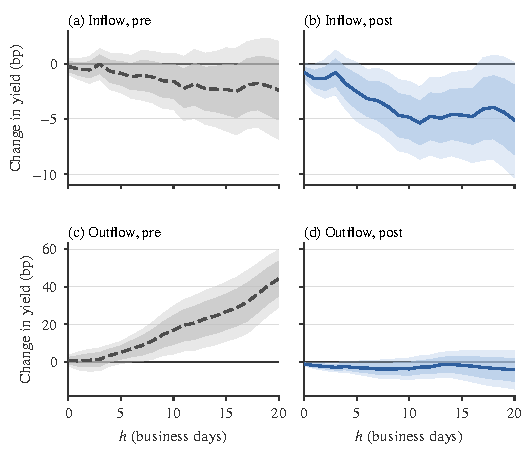
\includegraphics[width=\columnwidth]{figures/fig_asym.pdf}
\caption{Response of the 3-month bill yield to a USD~3.5\,bn five-day inflow (a,~b) and outflow (c,~d), before and after enactment. A positive outflow response means outflows raise yields. Rows share a vertical scale; 68\% and 90\% Newey--West bands.}
\label{fig:asym}
\end{figure}

\begin{table}[!t]
\centering
\caption{Asymmetry: response to a USD 3.5\,bn flow (bp, $p$)}
\label{tab:asym}
\footnotesize
\begin{adjustbox}{max width=\columnwidth}
% generated by src/viz/paper_tex.py
\begin{tabular}{lrrrr}
\toprule
Regime & $h$ & Inflow ($p$) & Outflow ($p$) & $p(\beta^-{=}\beta^+)$ \\
\midrule
Pre & 5 & \ensuremath{-}0.9 (0.41) & +5.0 (0.16) & 0.30 \\
 & 10 & \ensuremath{-}1.6 (0.30) & +16.9 (0.03) & 0.07 \\
 & 20 & \ensuremath{-}2.4 (0.37) & +44.3 ($<$0.01) & $<$0.01 \\
\midrule
Post & 5 & \ensuremath{-}2.6 (0.11) & \ensuremath{-}3.2 (0.13) & 0.05 \\
 & 10 & \ensuremath{-}4.9 (0.01) & \ensuremath{-}3.7 (0.28) & 0.05 \\
 & 20 & \ensuremath{-}5.1 (0.11) & \ensuremath{-}4.2 (0.50) & 0.22 \\
\bottomrule
\end{tabular}

\end{adjustbox}

\vspace{2pt}
\parbox{\columnwidth}{\footnotesize Inflow $=3.5\,\beta^+$; outflow $=-3.5\,\beta^-$. Last column: Wald test of $\beta^-=\beta^+$ within the regime.}
\end{table}

\subsection{Bill--policy-rate spread}

For the 3-month bill yield minus the effective federal funds rate, $\delta_{10}=\spDiff{}$\,bp (\spDiffP{}). Neither regime is significant (pre \spPre{}\,bp, \spPreP{}; post \spPost{}\,bp, \spPostP{}). The association with the bill yield is therefore not visible in the spread. This is consistent with the bill-yield association reflecting policy-rate expectations rather than a bill-specific scarcity premium, which would also explain why the controls-only estimate is larger than the instrumented one (Section~\ref{sec:discussion}).
